\documentclass[12pt,letterpaper]{article}
\usepackage{graphicx,textcomp}
\usepackage{natbib}
\usepackage{setspace}
\usepackage{fullpage}
\usepackage{color}
\usepackage[reqno]{amsmath}
\usepackage{amsthm}
\usepackage{fancyvrb}
\usepackage{amssymb,enumerate}
\usepackage[all]{xy}
\usepackage{endnotes}
\usepackage{lscape}
\newtheorem{com}{Comment}
\usepackage{float}
\usepackage{hyperref}
\newtheorem{lem} {Lemma}
\newtheorem{prop}{Proposition}
\newtheorem{thm}{Theorem}
\newtheorem{defn}{Definition}
\newtheorem{cor}{Corollary}
\newtheorem{obs}{Observation}
\usepackage[compact]{titlesec}
\usepackage{dcolumn}
\usepackage{tikz}
\usetikzlibrary{arrows}
\usepackage{multirow}
\usepackage{xcolor}
\newcolumntype{.}{D{.}{.}{-1}}
\newcolumntype{d}[1]{D{.}{.}{#1}}
\definecolor{light-gray}{gray}{0.65}
\usepackage{url}
\usepackage{listings}
\usepackage{color}
\usepackage{ dsfont }

\definecolor{codegreen}{rgb}{0,0.6,0}
\definecolor{codegray}{rgb}{0.5,0.5,0.5}
\definecolor{codepurple}{rgb}{0.58,0,0.82}
\definecolor{backcolour}{rgb}{0.95,0.95,0.92}

\lstdefinestyle{mystyle}{
	backgroundcolor=\color{backcolour},   
	commentstyle=\color{codegreen},
	keywordstyle=\color{magenta},
	numberstyle=\tiny\color{codegray},
	stringstyle=\color{codepurple},
	basicstyle=\footnotesize,
	breakatwhitespace=false,         
	breaklines=true,                 
	captionpos=b,                    
	keepspaces=true,                 
	numbers=left,                    
	numbersep=5pt,                  
	showspaces=false,                
	showstringspaces=false,
	showtabs=false,                  
	tabsize=2
}
\lstset{style=mystyle}
\newcommand{\Sref}[1]{Section~\ref{#1}}
\newtheorem{hyp}{Hypothesis}


\title{Problem Set 4}
\date{Due: November 18, 2024}
\author{Applied Stats/Quant Methods 1}


\begin{document}
	\maketitle
	\section*{Instructions}
	\begin{itemize}
		\item Please show your work! You may lose points by simply writing in the answer. If the problem requires you to execute commands in \texttt{R}, please include the code you used to get your answers. Please also include the \texttt{.R} file that contains your code. If you are not sure if work needs to be shown for a particular problem, please ask.
		\item Your homework should be submitted electronically on GitHub.
		\item This problem set is due before 23:59 on Monday November 18, 2024. No late assignments will be accepted.
	\end{itemize}



	\vspace{.5cm}
\section*{Question 1: Economics}
\vspace{.25cm}
\noindent 	
In this question, use the \texttt{prestige} dataset in the \texttt{car} library. First, run the following commands:

\begin{verbatim}
install.packages(car)
library(car)
data(Prestige)
help(Prestige)
\end{verbatim} 


\noindent We would like to study whether individuals with higher levels of income have more prestigious jobs. Moreover, we would like to study whether professionals have more prestigious jobs than blue and white collar workers.

\newpage
\begin{enumerate}
	
	\item [(a)]
	Create a new variable \texttt{professional} by recoding the variable \texttt{type} so that professionals are coded as $1$, and blue and white collar workers are coded as $0$ (Hint: \texttt{ifelse}).\\
	
	The dataset is imported as follows:
	\lstinputlisting[language=R, firstline=9, lastline=10]{PS04_Victor_Gomez_24362159.R}  
	
	and professional variable encoded into a binary one with:
	\lstinputlisting[language=R, firstline=11, lastline=14]{PS04_Victor_Gomez_24362159.R}  
	
	
	\item [(b)]
	Run a linear model with \texttt{prestige} as an outcome and \texttt{income}, \texttt{professional}, and the interaction of the two as predictors (Note: this is a continuous $\times$ dummy interaction.)
	
	The folowing line do the linear regression:
	\lstinputlisting[language=R, firstline=17, lastline=17]{PS04_Victor_Gomez_24362159.R}  	
	
	\begin{verbatim}
		> summary(lm1)

		Call:
		lm(formula = df$prestige ~ df$income + professional + df$income:professional)
		
		Residuals:
		    Min      1Q  Median      3Q     Max 
		-14.852  -5.332  -1.272   4.658  29.932 
		
		Coefficients:
		                         Estimate Std. Error t value Pr(>|t|)    
		(Intercept)            21.1422589  2.8044261   7.539 2.93e-11 ***
		df$income               0.0031709  0.0004993   6.351 7.55e-09 ***
		professional           37.7812800  4.2482744   8.893 4.14e-14 ***
		df$income:professional -0.0023257  0.0005675  -4.098 8.83e-05 ***
		---
		Signif. codes:  0 ‘***’ 0.001 ‘**’ 0.01 ‘*’ 0.05 ‘.’ 0.1 ‘ ’ 1
		
		Residual standard error: 8.012 on 94 degrees of freedom
		  (4 observations effacées parce que manquantes)
		Multiple R-squared:  0.7872,	Adjusted R-squared:  0.7804 
		F-statistic: 115.9 on 3 and 94 DF,  p-value: < 2.2e-16
	\end{verbatim}
	
	

	\item [(c)]
	Write the prediction equation based on the result.\\
	\\
	Considering $\hat{Y}$ the predictor of \texttt{prestige}, \\
			 $\hat{\beta_2}$ the slope along \texttt{income} ,\\
			$\hat{\beta_1}$ the slope along \texttt{professional} ,\\
			$\hat{\beta_{1,2}}$ the slope of calculated interaction ,\\
			 $\hat{\beta_0}$ the calculated intercept,\\
			 $X_2$ the  \texttt{income} variable\\ 
			$X_1$ the  \texttt{professional} variable \\
			 and the margin of error $\epsilon \leadsto  \mathcal{N} ( \mu, \sigma ), ( \mu, \sigma ) \in \mathds{R} \times \mathds{R}^+$, \\
			 the linear regression model gives:
			
			\begin{align*}
				 \hat{Y} &= \hat{\beta_2} X_2 + \hat{\beta_1} X_1+ \hat{\beta_{1,2}} X_1 X_2 + \hat{\beta_0} + \epsilon \\
				&=     0.003171   X_2 +  37.781280  X_1 - 0.002326 X_1 X_2 +  21.142259       + \epsilon
			\end{align*}
	
	\item [(d)]
	Interpret the coefficient for \texttt{income}.\\
	\\
	We have $\hat{\beta_2} \ll \hat{\beta_1}$ (by 4 orders of magnitude). So we can interpret this as $\hat{\beta_2} $ as neglectable. \\
	Although it cannot be rigorously considered as 0, since $\sigma_{\hat{\beta_2}}=0.0004993 < 0.1\hat{\beta_2}$ and the associated p-value is 6.351 7.55e-09. 
	I.e. \texttt{income} seems having an  influence on prestige, even if this one is small enough regarding other variations for being negected.

	\item [(e)]
	Interpret the coefficient for \texttt{professional}.\\
	\\
	We have$ \hat{\beta_1} =  37.781280 $ and $\sigma_{\hat{\beta_1}}= 4.2482744$ with a p-value of 4.14e-14. \\
	This means that  \texttt{professional} has a important impact on \texttt{prestige}. 
	
	\item [(f)]
	What is the effect of a \$1,000 increase in income on prestige score for professional occupations? In other words, we are interested in the marginal effect of income when the variable \texttt{professional} takes the value of $1$. Calculate the change in $\hat{y}$ associated with a \$1,000 increase in income based on your answer for (c).\\
	\\
		
	With the previous model plotted in Fig. \ref{fig:lm_1}., if professional is 1, the latter equation is simplified to:
	\begin{align*}
				 \hat{Y} &= \hat{\beta_2} X_2 + \hat{\beta_1} + \hat{\beta_{1,2}} X_2 + \hat{\beta_0} + \epsilon \\
				&=     0.003171   X_2 +  37.781280  - 0.002326 X_2 +  21.142259       + \epsilon
				&=   0.000845X_2 + 58,923539  +\epsilon
	\end{align*}

	\begin{figure}[h!]\centering
				\caption{\footnotesize Regression between \texttt{prestige} and  \texttt{income}}
				\label{fig:lm_1}
				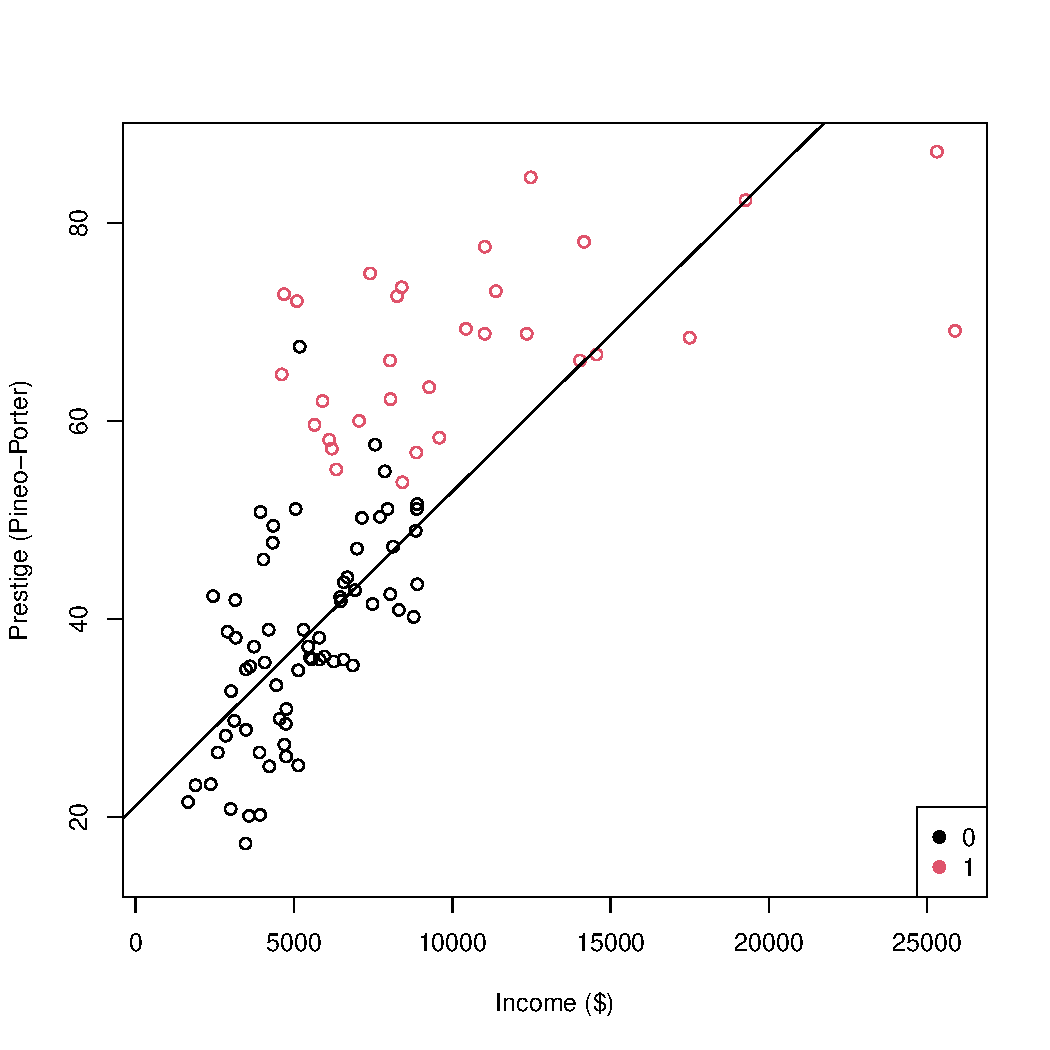
\includegraphics[width=.85\textwidth]{lm1.pdf}
	\end{figure}	
	We had at marginally for \texttt{income}:
	 $\frac{\partial \hat{Y}}{\partial X_2}= \hat{\beta_1} + \hat{\beta_{1,2}} = 0.000845$. \\
	Wich means, for a variation of income $\delta = \$1000$, the variation of prestige is\\
	 $\delta. \frac{\partial \hat{Y}}{\partial X_2}= \delta (\hat{\beta_1}+ \hat{\beta_{1,2}}) = 1000 \times 0.000845 = 0.0845$ points on Pineo-Porter prestige score. \\
	\\
	
	
	Note that this gives the same result if we consider from the beginning the bivariate regression between \texttt{prestige} and \texttt{income} for sample where \texttt{professional} is equal to 1, as follows:
		
	\begin{verbatim}
		summary(lm2)

		Call:
		lm(formula = ifelse(professional == 1, df$prestige, NA) ~ ifelse(professional == 
		    1, df$income, NA))
		
		Residuals:
		     Min       1Q   Median       3Q      Max 
		-12.2443  -5.1013  -0.5626   6.9908  15.1284 
		
		Coefficients:
		                                          Estimate Std. Error t value Pr(>|t|)    
		(Intercept)                              5.892e+01  2.985e+00   19.74  < 2e-16 ***
		ifelse(professional == 1, df$income, NA) 8.452e-04  2.523e-04    3.35  0.00226 ** 
		---
		Signif. codes:  0 ‘***’ 0.001 ‘**’ 0.01 ‘*’ 0.05 ‘.’ 0.1 ‘ ’ 1
		
		Residual standard error: 7.494 on 29 degrees of freedom
		  (71 observations effacées parce que manquantes)
		Multiple R-squared:  0.279,	Adjusted R-squared:  0.2541 
		F-statistic: 11.22 on 1 and 29 DF,  p-value: 0.002255
	\end{verbatim}	

	with this code:
	\lstinputlisting[language=R, firstline=20, lastline=20]{PS04_Victor_Gomez_24362159.R}  
	which plotted  gives Fig. \ref{fig:lm_2}
	\begin{figure}[h!]\centering
				\caption{\footnotesize Regression between \texttt{prestige} and  \texttt{income}}
				\label{fig:lm_2}
				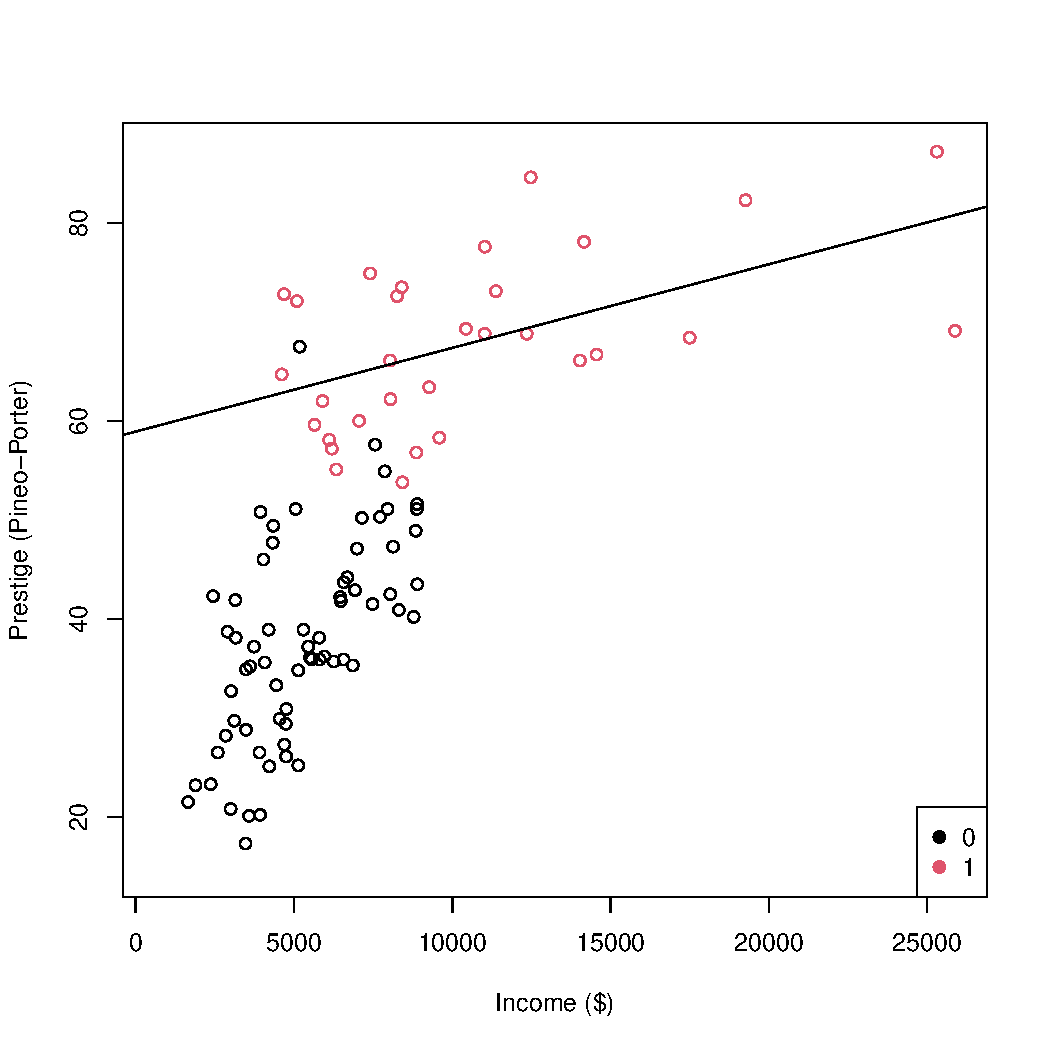
\includegraphics[width=.85\textwidth]{lm2.pdf}
	\end{figure}	

	This means that, using the same notations (which is accurate here since supposing $X_1=1$ leads to the simplified equation of the model above), we have:\\
	$\delta. \frac{\partial \hat{Y}}{\partial X_2}= \delta \hat{\beta_1} = 1000 \times 8.452e-04 = 0.8452$ points on Pineo-Porter (PPpt) prestige score with this second regression model. \\
	This is exactly the value found above. Note that the dispersion is smaller with this model (the standard deviation is ~2.5\%) compared to the first model (~5\% with the sum of
	 the two concerned coefficent standard deviation). The p-value is still reasonnable in this model (~2.3\%) even if its stronger with the first model ($10^{-8}$ and $10^{-4}$ ).

	\item [(g)]
	What is the effect of changing one's occupations from non-professional to professional when her income is \$6,000? We are interested in the marginal effect of professional jobs when the variable \texttt{income} takes the value of $6,000$. Calculate the change in $\hat{y}$ based on your answer for (c).\\
	\\
	For professional jobs, we have the folowing regression (cf. f.) :
	\begin{align*}
				 \hat{Y} &= (\hat{\beta_2} + \hat{\beta_{1,2}} )X_2 + (\hat{\beta_1} + \hat{\beta_0}) + \epsilon \\
				&=   0.000845X_2 + 58,923539  +\epsilon
	\end{align*}
	
	For non-professional occupations, we consider $X_1=0$, so
	\begin{align*}
				 \hat{Y} &= \hat{\beta_2} X_2 + \hat{\beta_1} X_1+  \hat{\beta_0} + \epsilon \\
				&=     0.003171   X_2 +  21.142259       + \epsilon
	\end{align*}
	In other words, the marginal effect on income variable is :\\
	$ m_p :=\frac{\partial \hat{Y}}{\partial X_2}=  \hat{\beta_1} = 8.452e-04 PPpt/\$$ for professional jobs, were as \\
	$ m_{np}:=\frac{\partial \hat{Y}}{\partial X_2}= \delta \hat{\beta_1} =  0.003171 PPpt/\$$ for non-professional jobs.\\
	i.e. the variation is reduced by $ m_p - m_{np} = 8.452e-04 -  0.003171 = - 0,002326 PPpt/\$$.
	
	
	
\end{enumerate}

\newpage

\section*{Question 2: Political Science}
\vspace{.25cm}
\noindent 	Researchers are interested in learning the effect of all of those yard signs on voting preferences.\footnote{Donald P. Green, Jonathan	S. Krasno, Alexander Coppock, Benjamin D. Farrer,	Brandon Lenoir, Joshua N. Zingher. 2016. ``The effects of lawn signs on vote outcomes: Results from four randomized field experiments.'' Electoral Studies 41: 143-150. } Working with a campaign in Fairfax County, Virginia, 131 precincts were randomly divided into a treatment and control group. In 30 precincts, signs were posted around the precinct that read, ``For Sale: Terry McAuliffe. Don't Sellout Virgina on November 5.'' \\

Below is the result of a regression with two variables and a constant.  The dependent variable is the proportion of the vote that went to McAuliff's opponent Ken Cuccinelli. The first variable indicates whether a precinct was randomly assigned to have the sign against McAuliffe posted. The second variable indicates
a precinct that was adjacent to a precinct in the treatment group (since people in those precincts might be exposed to the signs).  \\

\vspace{.5cm}
\begin{table}[!htbp]
	\centering 
	\textbf{Impact of lawn signs on vote share}\\
	\begin{tabular}{@{\extracolsep{5pt}}lccc} 
		\\[-1.8ex] 
		\hline \\[-1.8ex]
		Precinct assigned lawn signs  (n=30)  & 0.042\\
		& (0.016) \\
		Precinct adjacent to lawn signs (n=76) & 0.042 \\
		&  (0.013) \\
		Constant  & 0.302\\
		& (0.011)
		\\
		\hline \\
	\end{tabular}\\
	\footnotesize{\textit{Notes:} $R^2$=0.094, N=131}
\end{table}

\vspace{.5cm}
\begin{enumerate}
	\item [(a)] Use the results from a linear regression to determine whether having these yard signs in a precinct affects vote share (e.g., conduct a hypothesis test with $\alpha = .05$).\\
	\
	To test a hypothesis on the impact of lawn sign on vote share, a T-test on the associated coefficient has to be done. The null hypotesis is "This coefficent is equal to 0."
	 The p-value resulting from this test is given and is equal to 1.6\%. \\
	I.e. at risk 5\% ($>$ 1.6\%), the null hypotesis is rejected,\\
	i.e.   yard signs in a precinct affects vote share.
	
		
	\item [(b)]  Use the results to determine whether being
	next to precincts with these yard signs affects vote
	share (e.g., conduct a hypothesis test with $\alpha = .05$).\\
	\\
	To test a hypothesis on the impact of lawn sign in an adjacent precinct on vote share, a T-test on the associated coefficient has to be done. The null hypotesis is "This coefficent is equal to 0."
	 The p-value resulting from this test is given and is equal to 1.3\%. \\
	I.e. at risk 5\% ($>$1.3\%), the null hypotesis is rejected,\\
	i.e.   yard signs in an adjacent precinct affects vote share.
	
	\item [(c)] Interpret the coefficient for the constant term substantively.\\
	This coefficient represent the proportion of vote for McAuliff without lawn sign in a given precinct and its adjacent precincts (30.2\%).
	
	\item [(d)] Evaluate the model fit for this regression.  What does this tell us about the importance of yard signs versus other factors that are not modeled?\\
	\\ 
	It suffice to run an overall F-test on the proposed model. \\
	I.e. the test statistic $f=\frac{R^2/k}{(1-R^2)/(N-k-1)}=\frac{0.094/2}{(1-0.094)/(131-2-1)}=6.6$\\
	which gives the p-value 6.0\%.\\
	This is done with the following code:
	\lstinputlisting[language=R, firstline=48, lastline=51]{PS04_Victor_Gomez_24362159.R}  
	Considering a risk of 5\% the null hypotesis would not have been rejected.  In addition, the global $R^2=0.094$. I.e., les than 10\% of the variation is represented by this
	regression. In other words, there is other factors wich explain the remaining 90\% of the information.\\
	
	
\end{enumerate}  


\end{document}
